\section{Results}\label{sec:results}

All 24 Phase-1 sessions completed and were valid: no session exceeded the 25\,\%
infrastructure-error threshold, and none was quarantined. Reported energies are
NVML per-device integrals; accuracy is CIFAR-10 test-set accuracy measured once
per session on the best recipe the agent retained.

\subsection{Descriptive results}

\begin{table}[htbp]
\centering
\caption{Phase-1 session outcomes by proposer architecture ($n=12$ each).}
\label{tab:headline}
\begin{tabular}{lrrr}
\toprule
& dense 14B & MoE 30B-A3B & change \\
\midrule
Session GPU energy (kJ)      & 156.4 & \textbf{90.7} & $-42.0\,\%$ \\
Proposer energy (kJ)         &  94.3 & \textbf{35.7} & $-62.2\,\%$ \\
Training energy (kJ)         &  62.1 & 55.0 & $-11.4\,\%$ \\
Wasted energy (kJ)           & 126.1 & 67.0 & $-46.9\,\%$ \\
Test accuracy                & 0.7939 & \textbf{0.8224} & $+2.85$\,pp \\
Kept mutations (total)       & 12 & \textbf{17} & $+42\,\%$ \\
Sessions with zero kept      & 5/12 & 1/12 &, \\
Proposal latency (s)         & 61.8 & 31.9 & $-48.4\,\%$ \\
Session wall-clock (s)       & 1515 & 1023 & $-32.5\,\%$ \\
\bottomrule
\end{tabular}
\end{table}

\begin{figure}[htbp]
\centering
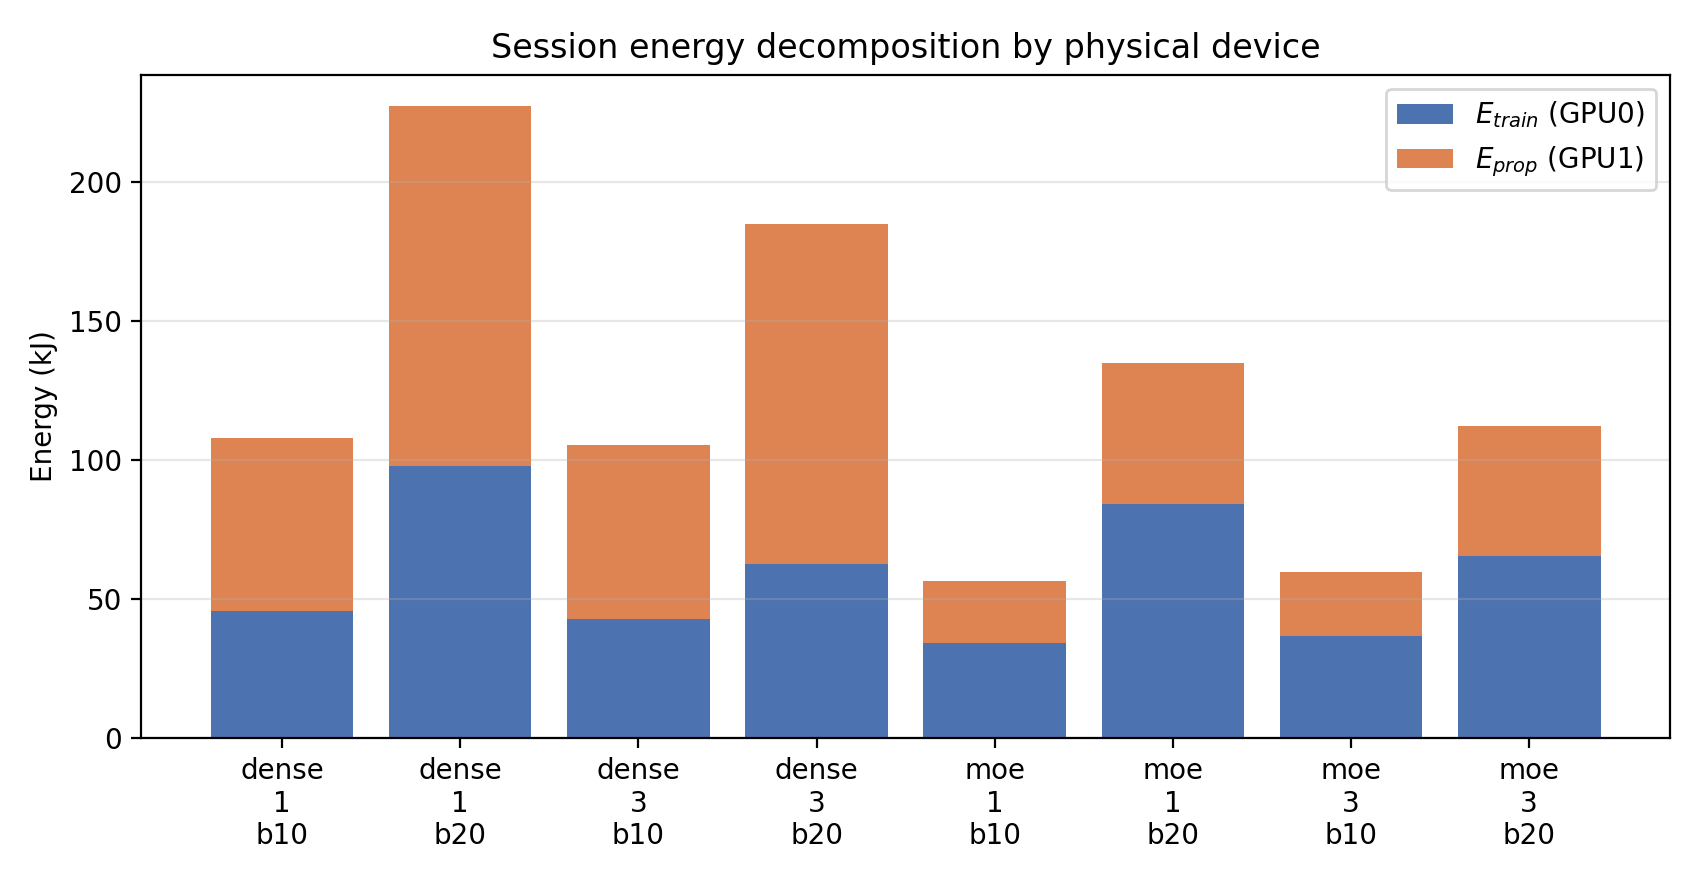
\includegraphics[width=\columnwidth]{figures/fig2_decomposition.png}
\caption{Session energy decomposed by physical device, per configuration cell.
Training energy (blue, GPU~0) is common to both arms and varies only with loop
budget; the architectural difference is concentrated almost entirely in proposer
energy (orange, GPU~1). This decomposition is a direct measurement, not an
estimate: the two components are read from separate devices.}
\label{fig:decomposition}
\end{figure}

Table~\ref{tab:headline} states the principal result: \textbf{the sparse proposer
is cheaper on every energy measure and more accurate}.
Figure~\ref{fig:decomposition} shows where the difference lives: the training
component is essentially identical across arms, as it must be, and the entire
architectural effect sits in the proposer component. This is not a trade-off
along a frontier; the MoE dominates. The mechanism is multiplicative: activating
$\sim$3B rather than 14.8B parameters draws $\sim$36\,\% less instantaneous power
(72.5\,W vs.\ 112.8\,W measured during proposal phases) \emph{and} completes a
proposal in half the time.

\begin{figure*}[htbp]
\centering
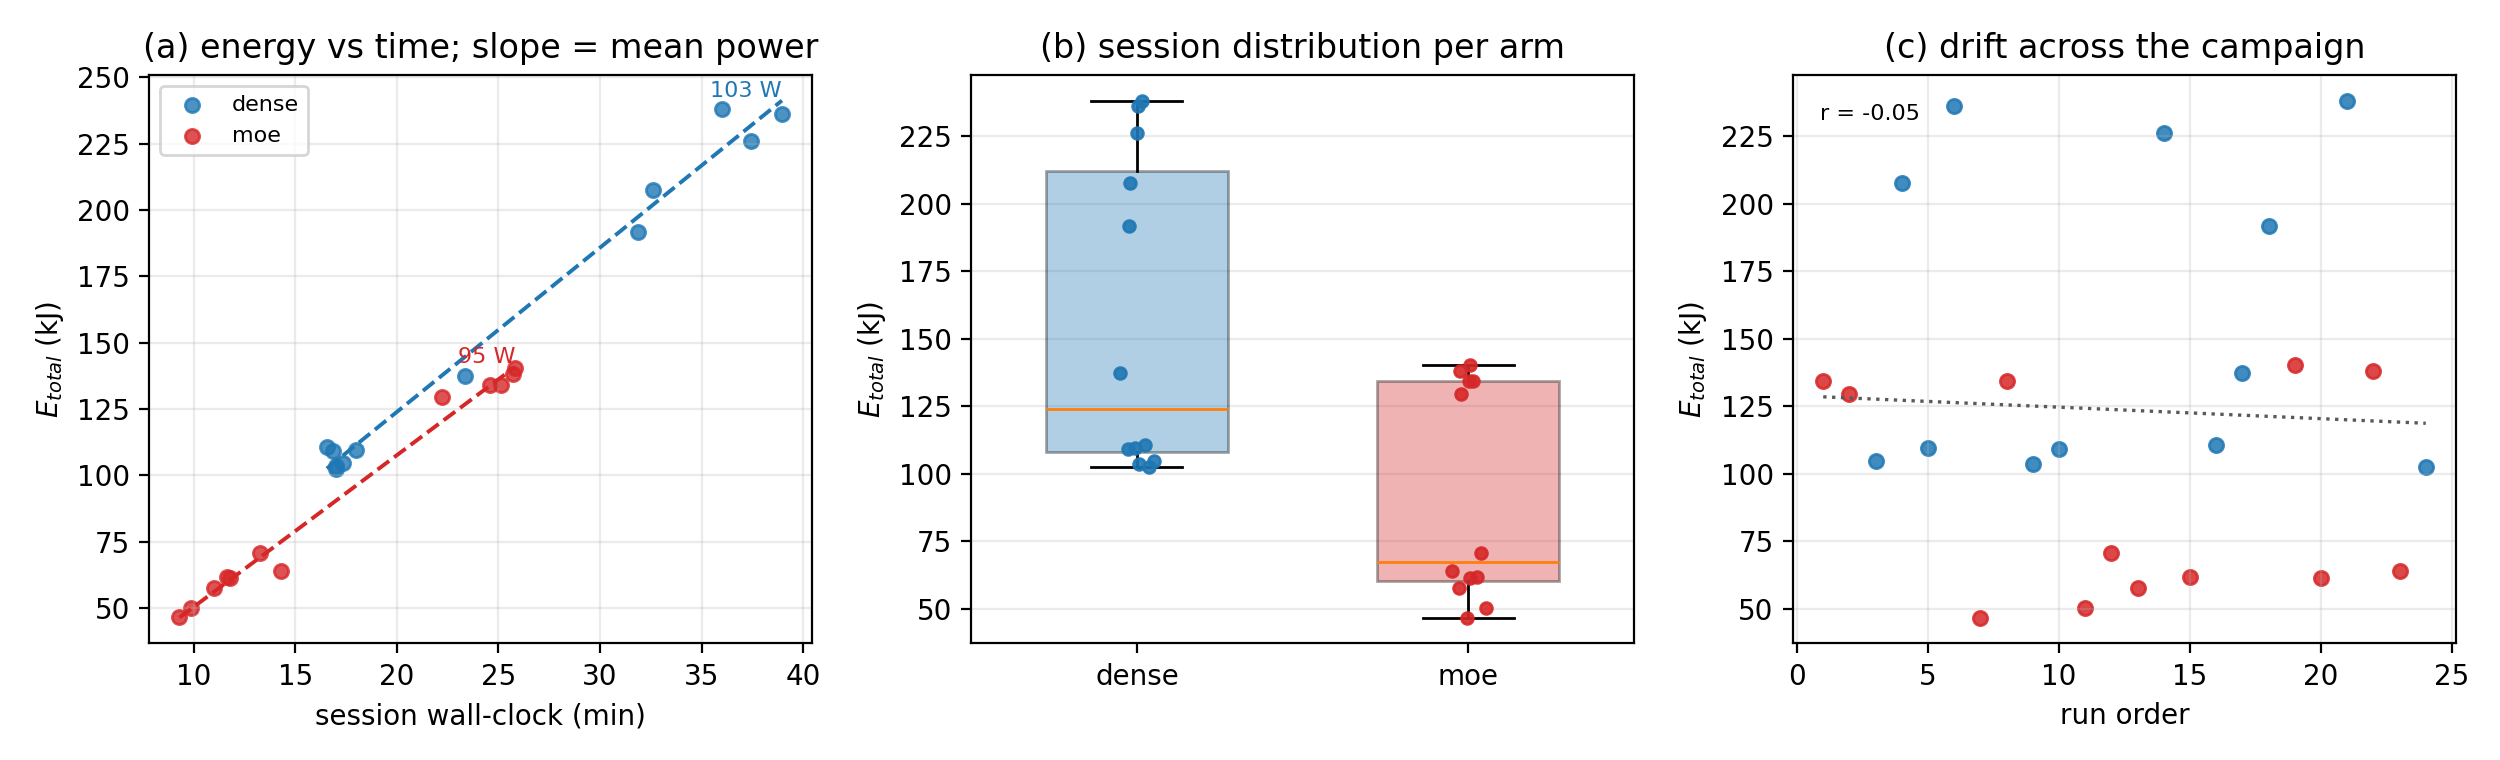
\includegraphics[width=\textwidth]{figures/fig6_diagnostics.png}
\caption{Measurement diagnostics. (a) Session energy against wall-clock; the
fitted slope is mean session power. (b) Session-level distributions per arm.
(c) Session energy against position in the randomised run table.}
\label{fig:diagnostics}
\end{figure*}

\textbf{Is this simply a speed result?} Figure~\ref{fig:diagnostics}(a) separates
the two components. Mean \emph{session} power differs by only 16\,\% between the
arms (103\,W dense, 95\,W MoE) because both share an identically loaded training
GPU; session duration differs by 48\,\%. The energy ratio decomposes as
$1.48 \times 1.16 = 1.72$, i.e.\ roughly two thirds of the session-level
advantage is shorter sessions and one third is lower power. The large power
difference is real but confined to the component the architecture governs: during
proposal phases the devices draw 112.8\,W (dense) against 72.5\,W (MoE), and
$E_{\mathit{prop}}$ per proposal differs by $2.7\times$. Reporting only session
energy would understate the architectural effect; reporting only proposer power
would overstate it.

Figure~\ref{fig:diagnostics}(c) addresses run order: energy correlates with
position in the run table at $r = -0.05$, so no thermal or environmental drift
accumulated across the campaign that randomisation would have needed to absorb.

\subsection{RQ1: effects of configuration on the energy/accuracy profile}

Shapiro--Wilk rejected normality for session energy ($W=0.889$, $p=0.012$) while
Levene's test found homoscedasticity ($p=0.46$), so the Aligned Rank Transform
was applied before ANOVA.

\begin{table}[htbp]
\centering
\caption{ART-ANOVA on session GPU energy.}
\label{tab:anova}
\begin{tabular}{lrrr}
\toprule
Effect & $F$ & $p$ & partial $\eta^2$ \\
\midrule
Proposer            & 42.61 & $6.96\times10^{-6}$ & \textbf{0.727} \\
Loop budget         & 50.58 & $2.47\times10^{-6}$ & \textbf{0.760} \\
Patience            &  2.77 & 0.116 & 0.147 \\
Proposer $\times$ patience     & 0.70 & 0.416 & 0.042 \\
Proposer $\times$ loop budget  & $\approx$0 & 1.000 & $\approx$0 \\
Patience $\times$ loop budget  & 1.39 & 0.256 & 0.080 \\
\bottomrule
\end{tabular}
\end{table}

\begin{table}[htbp]
\centering
\caption{Pre-registered contrasts. Mann--Whitney $U$, Cliff's $\delta$, Holm
correction over five tests.}
\label{tab:contrasts}
\begin{tabular}{llrlr}
\toprule
Hypothesis & Outcome & Change & Cliff's $\delta$ & $p_{\mathit{holm}}$ \\
\midrule
H$^{\mathit{prop}}$ & $E_{\mathit{total}}$   & $-42.0\,\%$ & 0.556 (large)      & 0.090 \\
H$^{\mathit{prop}}$ & test acc.              & $+3.6\,\%$  & $-0.444$ (medium)  & 0.207 \\
H$^{\mathit{bud}}$  & $E_{\mathit{per\,kept}}$ & $+107.6\,\%$ & $-0.802$ (large) & \textbf{0.024} \\
H$^{\mathit{pat}}$  & $E_{\mathit{wasted}}$  & $-9.8\,\%$  & 0.042 (negligible) & 1.000 \\
H$^{\mathit{pat}}$  & $E_{\mathit{per\,kept}}$ & $-9.4\,\%$ & 0.117 (negligible) & 1.000 \\
\bottomrule
\end{tabular}
\end{table}

Proposer architecture and loop budget both carry large effects on session energy
($\eta^2_p = 0.73$ and $0.76$); patience does not, and no interaction is
detectable. Consistent with the conclusion-validity position registered in
Section~\ref{sec:threats}, \textbf{effect sizes are the primary output}. The
architecture effect is unambiguous under ART-ANOVA ($p = 7\times10^{-6}$) while
the corresponding pairwise contrast does not survive Holm correction
($p_{\mathit{holm}} = 0.090$). These are not in conflict: the ANOVA models loop
budget, itself a large energy effect, whereas the pairwise test pools across it
and inherits that variance. With $n=12$ per arm the defensible claim is a large
and consistent effect that the corrected pairwise test is underpowered to certify
at $\alpha = 0.05$.

Doubling the loop budget from 10 to 20 raised energy per kept mutation by
$107.6\,\%$ ($\delta = -0.80$, the only Holm-significant contrast): twice the
experiments cost twice the energy per useful result, because the cheap
improvements are found early in a session.

\begin{figure}[htbp]
\centering
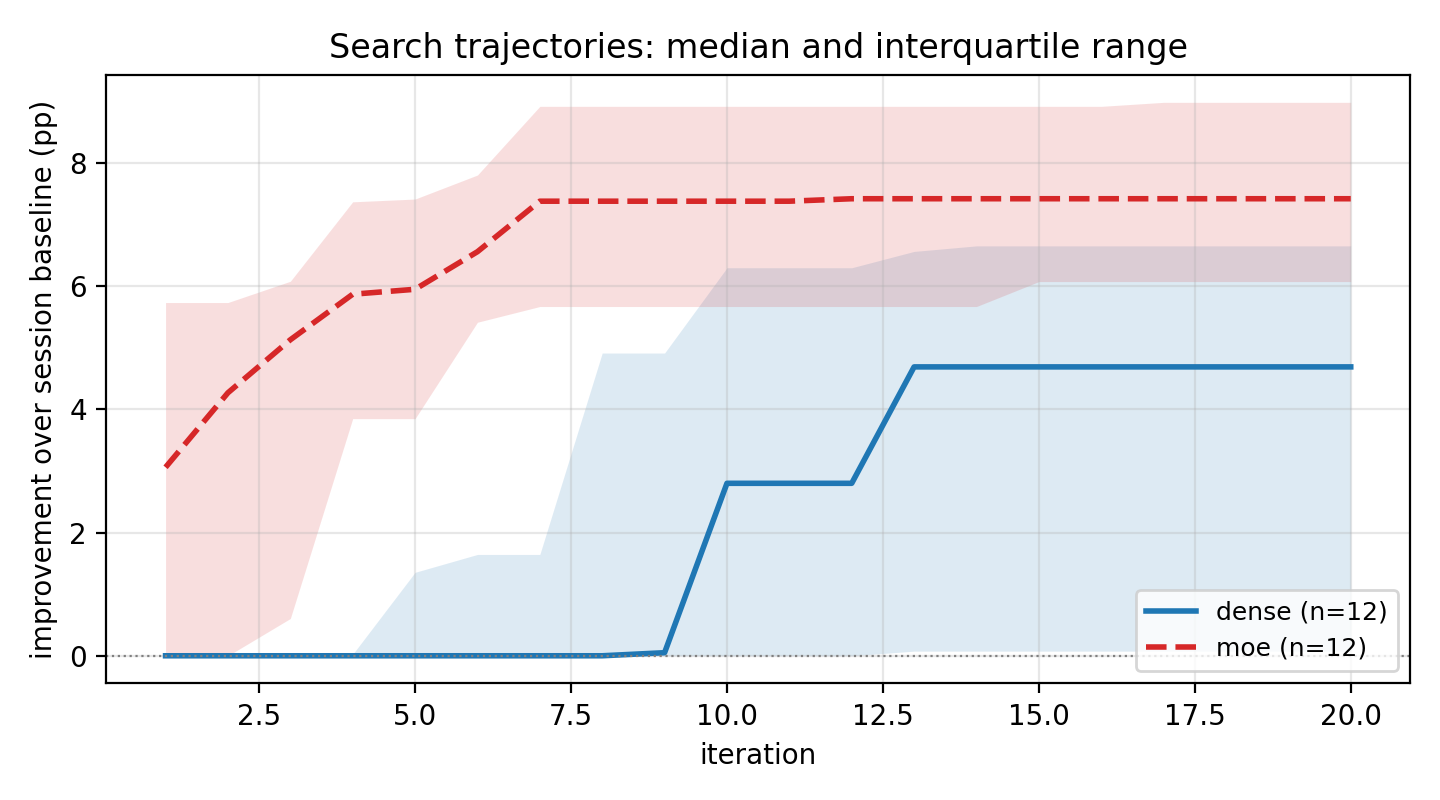
\includegraphics[width=\columnwidth]{figures/fig5_trajectories.png}
\caption{Improvement over each session's own baseline, median with
interquartile band, $n=12$ sessions per arm. Curves are monotone by
construction: a proposal that fails to improve is reverted. The MoE reaches
$+3$\,pp by its first iteration and plateaus near $+7.4$\,pp by iteration~7; the
dense arm's median is flat until iteration~9 and plateaus lower.}
\label{fig:trajectories}
\end{figure}

Figure~\ref{fig:trajectories} shows the mechanism directly, and adds a
distinction the aggregate tables cannot: the two arms differ not only in how much
they improve but in \emph{when}. The MoE's median session has gained $+3$\,pp
after a single iteration and has essentially finished by iteration~7, whereas the
dense median does not move until iteration~9. Sessions reach their final recipe
early and spend the remaining iterations proposing alternatives that are
rejected; that energy is not recovered.

\begin{figure}[htbp]
\centering
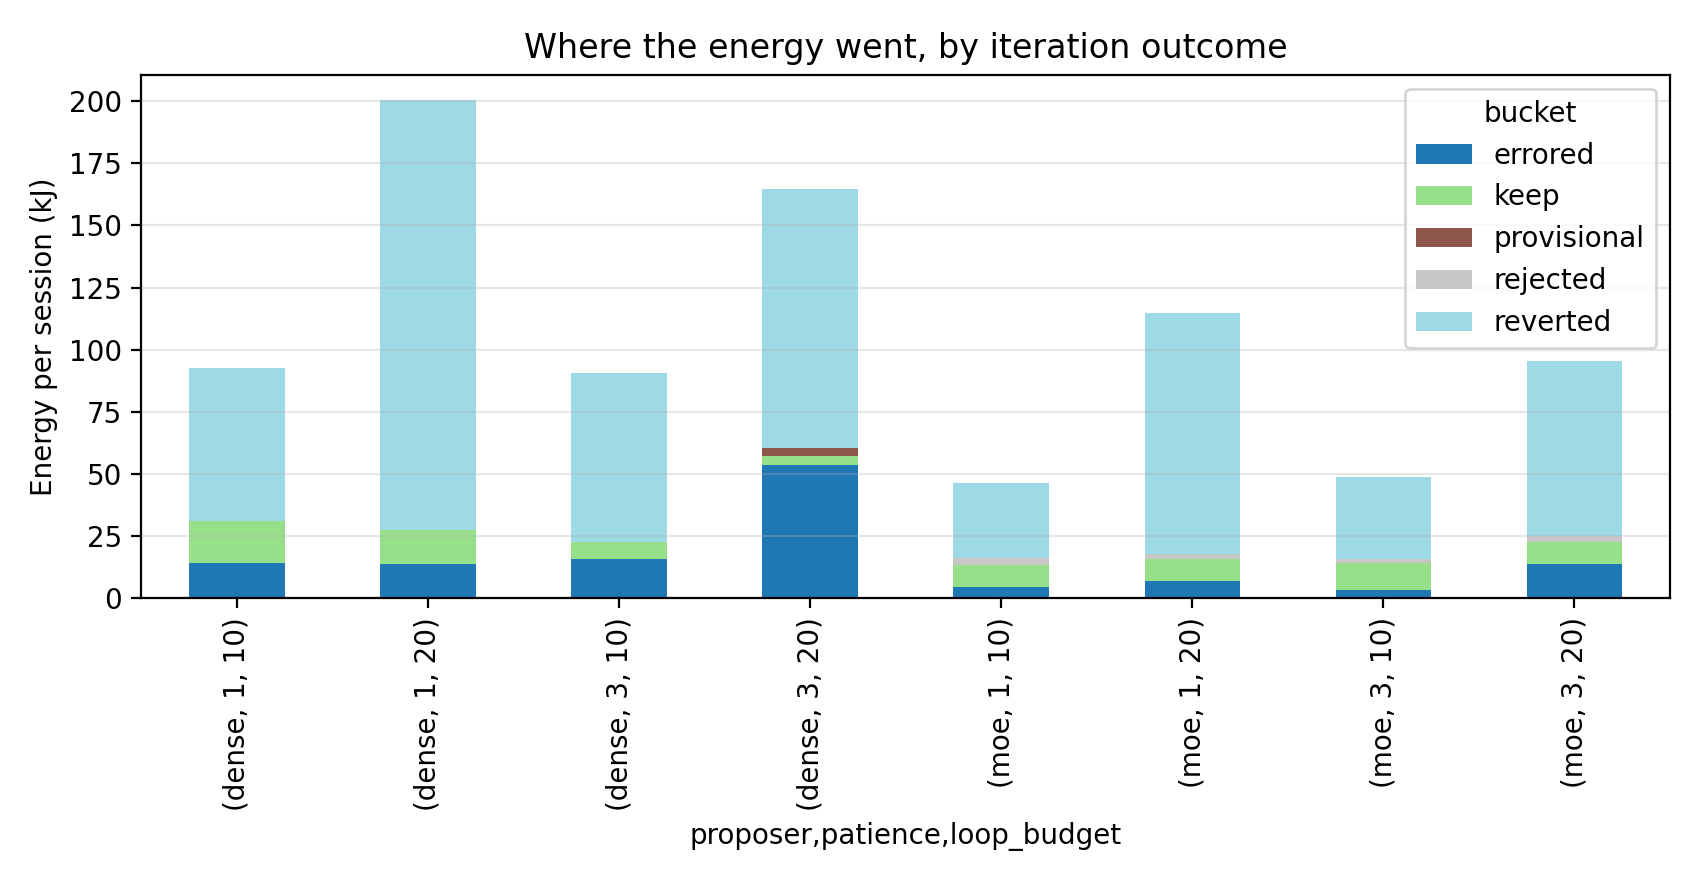
\includegraphics[width=\columnwidth]{figures/fig4_waste.png}
\caption{Per-session energy attributed to each iteration outcome. The
\emph{keep} band is small in every cell: 64\,\% of Phase-1 session energy went to
mutations that were reverted or that failed to run. This is a property of the
protocol rather than a defect, a search must evaluate candidates to
reject them, and it is precisely what makes proposer efficiency worth
measuring.}
\label{fig:waste}
\end{figure}

Figure~\ref{fig:waste} attributes that energy by outcome. Across Phase~1,
\textbf{64\,\% of session energy produced no retained mutation}, and the dense
arm wasted 126.1\,kJ per session against the MoE's 67.0\,kJ.

\subsection{RQ2: the energy/accuracy Pareto frontier}

\begin{table}[htbp]
\centering
\caption{Cell means and the non-dominated frontier.}
\label{tab:pareto}
\begin{tabular}{llrrrc}
\toprule
Proposer & Pat. & Bud. & $E$ (kJ) & Test acc. & Frontier \\
\midrule
MoE   & 1 & 10 & \textbf{56.5} & 0.8209 & yes \\
MoE   & 3 & 10 & 59.5 & 0.8134 & \\
dense & 3 & 10 & 105.4 & 0.7729 & \\
dense & 1 & 10 & 107.9 & 0.8214 & yes$^\dagger$ \\
MoE   & 3 & 20 & 112.0 & \textbf{0.8311} & yes \\
MoE   & 1 & 20 & 134.7 & 0.8242 & \\
dense & 3 & 20 & 185.0 & 0.7763 & \\
dense & 1 & 20 & 227.3 & 0.8049 & \\
\bottomrule
\end{tabular}
\end{table}

\begin{figure}[htbp]
\centering
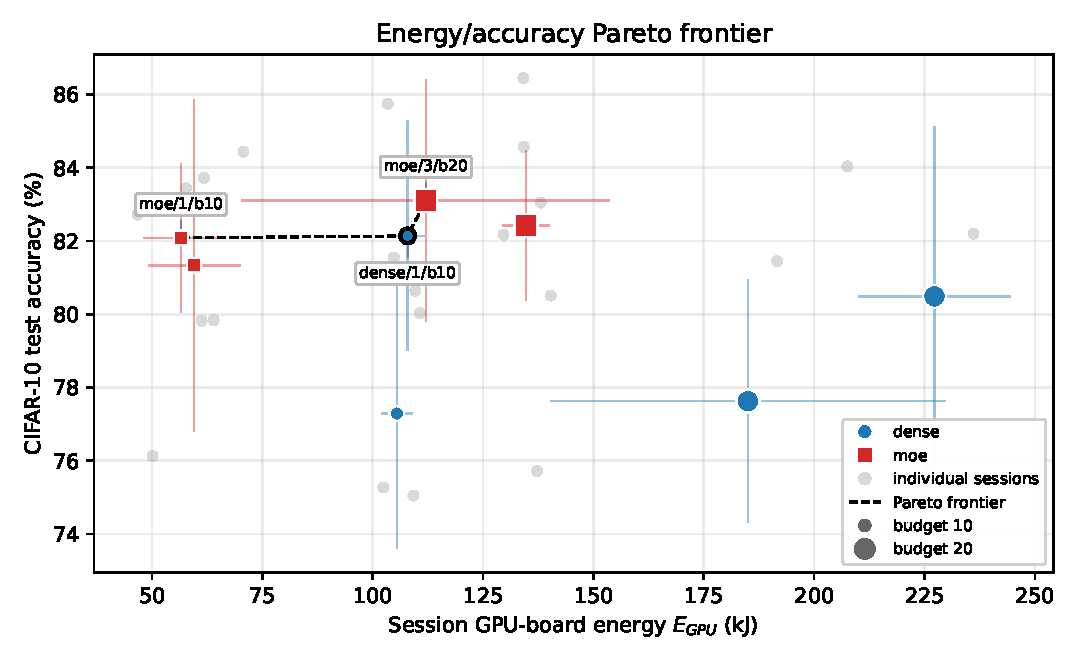
\includegraphics[width=\columnwidth]{figures/fig1_pareto.pdf}
\caption{Energy/accuracy Pareto frontier. Large markers are cell means with
$\pm$1\,SD bars; small grey points are individual sessions. Marker shape encodes
proposer, colour encodes patience, size encodes loop budget, and the designated
baseline cell (dense, greedy, budget~10) is outlined. The within-cell spread is
substantial relative to the between-cell differences in accuracy, which is why
frontier membership is interpreted against the measured noise floor rather than
from means alone.}
\label{fig:pareto}
\end{figure}

Two of the three non-dominated cells are MoE cells, and the cheapest frontier
point (MoE, greedy, budget 10) attains 0.8209 test accuracy for 56.5\,kJ,
\textbf{47.6\,\% less energy than the designated baseline cell} (dense, greedy,
budget~10) at 0.05\,pp lower mean accuracy, i.e.\ at no measurable accuracy cost., 
Figure~\ref{fig:pareto} also makes the dispersion visible: within-cell spread is
large relative to between-cell accuracy differences, which is the reason the
frontier is read against the noise floor below.

\textbf{The dense frontier point ($\dagger$) is an artifact of measurement noise
and should not be read as a genuine trade-off.} It is non-dominated only because
its mean accuracy exceeds the cheapest MoE cell by $0.053$\,pp, 23 times
smaller than the measured keep threshold ($\epsilon = 1.23$\,pp,
Section~\ref{sec:execution}) and 60 times smaller than the within-cell standard
deviation ($3.1$\,pp), while consuming $1.91\times$ the energy. A frontier
computed from cell means without reference to the noise floor will report
spurious non-dominated points; we therefore report each frontier margin against
$\epsilon$.

\subsection{Reliability of improvement}

\begin{table}[htbp]
\centering
\caption{Best accuracy \emph{observed} within a session, relative to that
session's own baseline (retained regardless of the keep decision).}
\label{tab:reliability}
\begin{tabular}{lrr}
\toprule
& Mean & Median \\
\midrule
dense 14B    & $-2.21$\,pp & $+4.69$\,pp \\
MoE 30B-A3B  & $+7.23$\,pp & $+7.42$\,pp \\
\bottomrule
\end{tabular}
\end{table}

The dense arm's mean is negative while its median is positive: a minority of
sessions collapse catastrophically, individual proposals reached $0.0924$
validation accuracy, chance level for ten classes, and pull the mean below
baseline. The MoE's mean and median nearly coincide.

\textbf{The architectural difference is therefore one of reliability as much as
of quality.} For a self-hoster this is the more consequential property: a session
that ends below its own baseline has spent its entire energy budget for a
negative result. We report best-observed accuracy alongside best-kept accuracy
because the latter collapses to the baseline whenever no proposal clears
$\epsilon$, and carries no signal in those sessions.

\subsection{Energy per kept mutation: reporting convention}

$E_{\mathit{per\,kept}}$ is undefined for a session that keeps nothing, and 5 of
12 dense sessions kept nothing (against 1 of 12 for the MoE; Fisher exact
$p=0.155$). The choice of convention materially changes the reported effect:

\begin{table}[htbp]
\centering
\caption{Two conventions for energy per kept mutation.}
\label{tab:perkept}
\small
\begin{tabular}{lrrr}
\toprule
Convention & dense & MoE & ratio \\
\midrule
Mean of ratios$^\dagger$ & 112.1\,kJ & 74.4\,kJ & $1.51\times$ \\
Pooled $\sum E / \sum \mathit{kept}$ & \textbf{156.4}\,kJ & \textbf{64.0}\,kJ & $\mathbf{2.44\times}$ \\
\bottomrule
\end{tabular}
\par\smallskip
{\footnotesize $^\dagger$ mean of the per-session ratios, which necessarily
excludes sessions that kept nothing.}
\end{table}

The first convention understates the effect by 38\,\% precisely because it
discards the sessions in which the dense arm performed worst. We report the
pooled figure and state the zero-kept counts alongside it.

\subsection{Agent behaviour}

\textbf{Contract compliance and proposal quality are independent axes.} The
guard rejected 0.0\,\% of dense proposals and 9.6\,\% of MoE proposals (maximum
30\,\% in one session), yet the MoE produced the better recipes. A benchmark
scoring only output-format compliance would rank these two models in the opposite
order. The same dissociation appeared in the pilot, where a 4B model was rejected
on four of six iterations and still gained $+8.8$\,pp while a 14B model complied
perfectly and gained nothing.

\textbf{Failure to run is a dependent variable.} Sessions averaged 4.1 (dense) and
3.3 (MoE) crashed proposals, with single-session extremes of 19/20 and 15/20.
Because a crashed proposal consumes a full proposer inference and returns
nothing, crash rate feeds directly into energy efficiency. A representative
failure: the dense proposer replaced
\texttt{SGD} at \texttt{lr=0.01} with \texttt{AdamW} at the same rate, retaining a
learning rate roughly an order of magnitude too large for Adam, and reached
$0.0924$ accuracy.

\textbf{Thinking mode was verified, not assumed.} Summing reasoning tokens over
all 360 proposals in both arms yields zero, confirming that
\texttt{enable\_thinking:\,false} was honoured by the serving stack rather than
merely accepted.

\subsection{Stage 2a: does reasoning pay for itself?}\label{sec:results:reasoning}

Reasoning mode is a fixed variable in Stage~1 (disabled for both arms, verified
at zero tokens across all 360 Phase-1 proposals). Stage~2a promotes it to a
factor: \texttt{proposer} $\times$ \texttt{thinking}, 3 repetitions, greedy,
budget~10. All 12 sessions were valid. The manipulation is confirmed by
measurement rather than by configuration: every \texttt{off} session emitted
exactly 0 reasoning tokens and every \texttt{on} session between 23\,909 and
47\,904.

\begin{table}[htbp]
\centering
\caption{Stage 2a cells ($n=3$ each).}
\label{tab:reasoning}
\begin{tabular}{llrrrrr}
\toprule
Arm & Think & $E$ (kJ) & $E_{\mathit{prop}}$ & Test acc. & Kept & Err. \\
\midrule
dense & off & 108.1 & 59.2  & 0.7572 & 0.33 & 1.0 \\
dense & on  & 172.6 & 133.3 & 0.8490 & 1.33 & 4.3 \\
MoE   & off & \textbf{52.1} & \textbf{22.0} & 0.8469 & \textbf{2.00} & 3.3 \\
MoE   & on  & 92.0  & 59.0  & 0.8378 & 1.00 & 4.3 \\
\bottomrule
\end{tabular}
\end{table}

\begin{figure}[htbp]
\centering
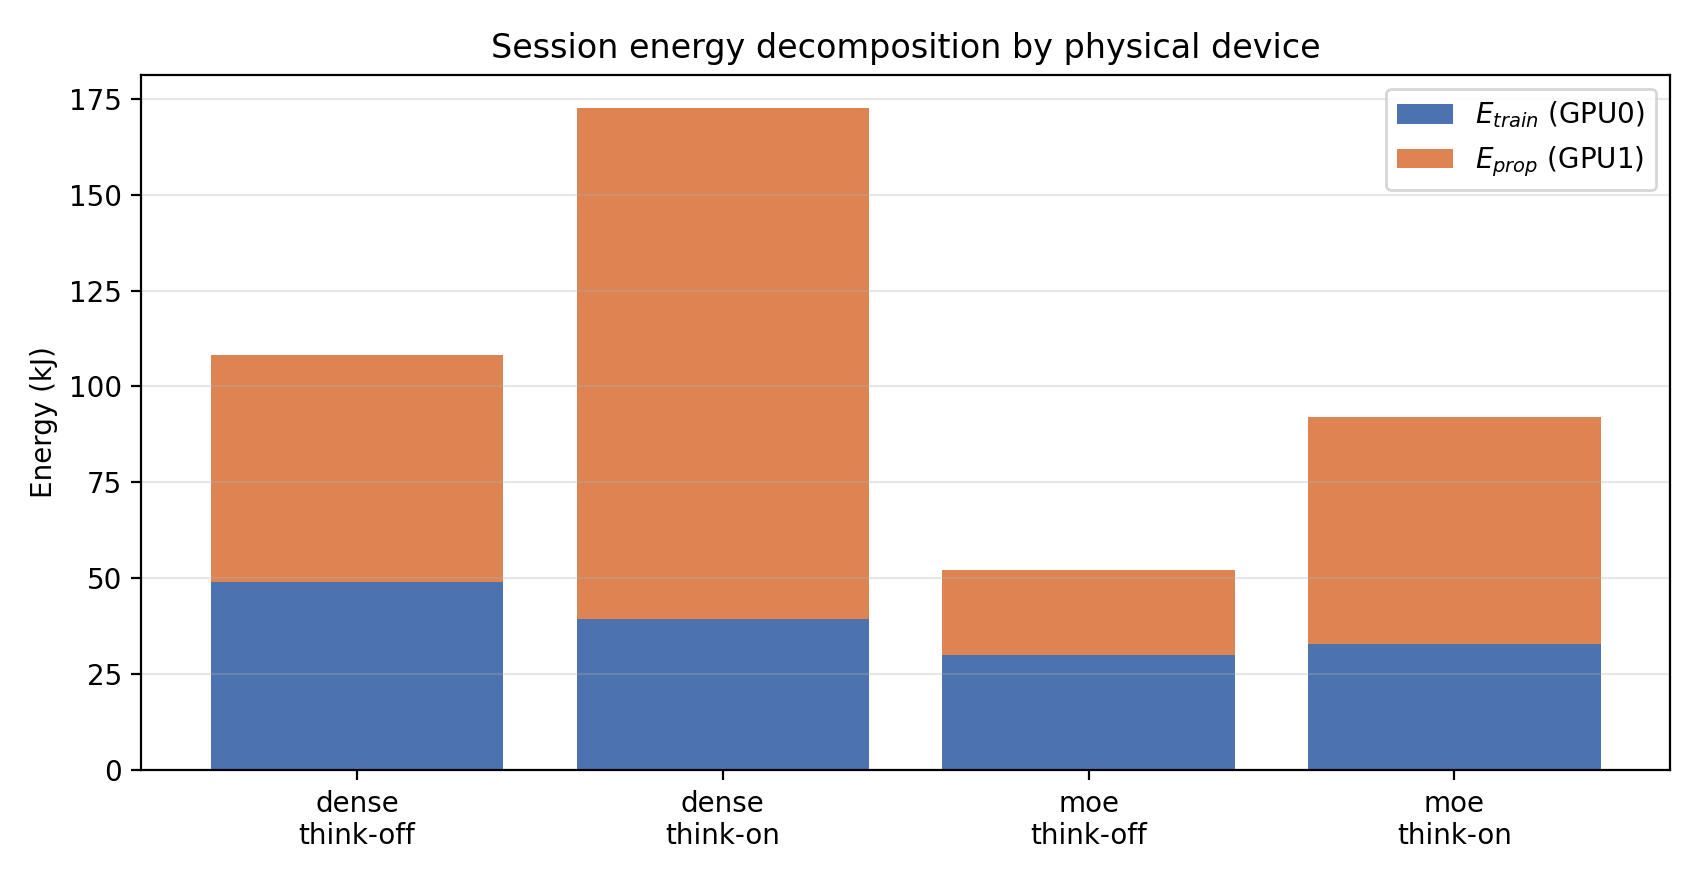
\includegraphics[width=\columnwidth]{figures/fig3_reasoning_decomposition.png}
\caption{Stage 2a: session energy by device. Reasoning inflates the proposer
component (orange) while leaving training (blue) unchanged, as it must. The two
configurations that matter are the extremes: \emph{MoE without reasoning} at
52\,kJ and \emph{dense with reasoning} at 173\,kJ, which reach statistically
indistinguishable accuracy.}
\label{fig:reasoning}
\end{figure}

\textbf{Reasoning and sparsity are substitutes, not complements.} Enabling
reasoning raises dense test accuracy substantially but leaves the MoE unchanged:
the MoE difference of $0.91$\,pp lies below the measured keep threshold
($\epsilon = 1.23$\,pp) and is not interpretable as an effect. Pooling the two
independent executions of the dense-without-reasoning configuration
(Section~\ref{sec:results:control}, $n=6$) puts the dense gain at $+6.0$\,pp.

\textbf{The practitioner reading inverts the intuitive one.} The cheapest
configuration measured, MoE without reasoning, attains 0.8469 test accuracy for
52.1\,kJ, against dense with reasoning at 0.8490 for 172.6\,kJ: \textbf{3.3
times less energy for an accuracy difference of 0.21\,pp}, six times smaller than
the noise floor. On a fixed energy budget, sparsity is the efficient purchase and
reasoning tokens are not; reasoning is an expensive route to a point the sparse
model reaches without it.

We registered a quantitative prediction before running, derived from the
feasibility probe and the measured proposal-phase power draws: that the MoE could
reason for less energy than the dense model spends not reasoning (6.17 vs.\
6.73\,kJ per proposal). The direction held and the absolute values fell within
5\,\% of prediction (5.90 vs.\ 5.92\,kJ), but the margin collapsed from 0.56 to
0.02\,kJ. The defensible claim is equality, not inequality.

Finally, reasoning did \emph{not} reduce coding errors: failures per session rose
in both arms (dense 1.0~$\rightarrow$~4.3, MoE 3.3~$\rightarrow$~4.3). We had
expected a reasoning pass to catch errors such as retaining an SGD learning rate
when switching to AdamW. It did not; longer deliberation produced more ambitious
proposals rather than more correct ones.

\subsection{A reproducibility control}\label{sec:results:control}

Phase~1's \emph{dense, greedy, budget-10} cell and Stage~2a's \emph{dense,
reasoning-off} cell are the same configuration, executed in independent
experiments days apart on the same hardware. They therefore function as an
unplanned replication.

\begin{table}[htbp]
\centering
\caption{The same configuration, executed twice independently.}
\label{tab:control}
\begin{tabular}{lrrl}
\toprule
& Phase 1 & Stage 2a & Agreement \\
\midrule
Session energy & 107.9\,kJ & 108.1\,kJ & \textbf{0.20\,\%} \\
Test accuracy  & 0.8214 & 0.7572 & 6.42\,pp apart \\
Kept mutations & 1.67 & 0.33 &, \\
\bottomrule
\end{tabular}
\end{table}

\textbf{Energy reproduces to a fifth of a percent; accuracy does not reproduce at
$n=3$.} The measurement apparatus is thus not the source of the accuracy
variance; the agent is. This is the clearest available justification for the
conclusion-validity position registered in Section~\ref{sec:threats}, that effect
sizes rather than significance tests are the primary output, and it is a concrete
warning against reading any individual three-session cell as a point estimate of
accuracy. It also implies that the energy comparisons in this study are
considerably better powered than the accuracy comparisons and should carry
correspondingly more of the argument.

\subsection{Stage 2b: sampling temperature, and a correction}\label{sec:results:temperature}

Phase~1 was restarted once because its first three sessions kept no mutations at
all, which we attributed at the time to sampling temperature 0 making the search
degenerate. Stage~2b tests that attribution directly: four temperatures, three
repetitions, MoE arm, against the current prompt.

\begin{table}[htbp]
\centering
\caption{Stage 2b: sampling temperature, MoE arm ($n=3$ per level).}
\label{tab:temperature}
\small
\begin{tabular}{rrrrrr}
\toprule
$T$ & $E$ (kJ) & Test acc. & Kept & Duplicate pairs & Distinct \\
\midrule
0.0 & 65.8 & 0.8289 & 1.67 & 23 & 0.77 \\
0.4 & 65.6 & 0.8222 & 1.67 & 5  & 0.90 \\
0.7 & 55.4 & 0.8137 & 1.33 & 2  & 0.97 \\
1.0 & 66.0 & 0.8173 & 2.33 & 9  & 0.87 \\
\bottomrule
\end{tabular}
\end{table}

\textbf{Temperature changes proposal duplication but not outcomes.} Byte-identical
proposal pairs fall from 23 at $T=0$ to between 2 and 9 above it, and the fraction
of distinct proposals within a session rises from 0.77 to 0.97. Retained
mutations (1.33--2.33) and best observed accuracy (0.8235--0.8361) show no
corresponding pattern. One $T=0$ session produced only 4 distinct proposals out of
10 and still retained 2 mutations, reaching 0.8486. Duplicate proposals waste
iterations; on this evidence they do not prevent a session from succeeding.

\textbf{The original attribution was wrong.} At $T=0$ against the current prompt
the MoE retains 1.67 mutations per session, which is the normal rate for that
arm. Temperature 0 therefore does not produce sessions that retain nothing, and
cannot by itself explain the restarted Phase~1.

Two other findings account for what we saw. First, the three sessions that
prompted the restart were, by the shuffled run order, all dense
($P = 0.11$ for the first three runs of a balanced 24-row table). Second, the
dense arm retains nothing in 5 of its 12 Phase-1 sessions even at $T=0.7$ with
the corrected prompt, a rate of 0.42. Three consecutive zero-retention dense
sessions is therefore an ordinary draw rather than evidence of a broken search.

\textbf{What the prompt did.} The restart also added a measured statement of the
training budget to the prompt. That change is not neutral, but its effect is
arm-specific: of the dense arm's \texttt{T\_max} literals in Stage 2a, 19 of 20
still specify more than 60 epochs for a budget that delivers roughly 43, whereas
the MoE emits none out of 82 in Stage 2b. The dense proposer continues to design
for a training run it is not given, after being told what it is given.

\textbf{Limits of this correction.} Stage 2b varies temperature on the MoE only,
so we have not tested $T=0$ on the dense arm against the corrected prompt. What
we can state is that the mechanism we proposed does not operate on the arm we
tested, that temperature has no detectable effect on any outcome over $[0, 1]$,
and that the observation which triggered the restart is adequately explained
without it.
